\chapter{Forschungsdesign}
\label{kap:forschungsdesign}
Das Hauptziel der Arbeit ist das Erstellen eines Visual-Analytics-Tools, mithilfe dessen Trends und Anomalien aufgrund von Verspätungen im \acrshort{sbb} Zugnetzwerk exploriert werden können. Das Vorgehen orientiert sich hierbei an der Visualisierungspipeline von Chen et al. (siehe Abbildung \ref{fig_pipeline_traffic_visualization}), fügt jedoch noch zusätzliche Schritte wie UI-Design, Algorithmen sowie Performance-Analyse hinzu (siehe Abbildung \ref{fig_vorgehen}).

\begin{figure}[H]
    \caption{Vorgehensweise (eigene Darstellung)}
    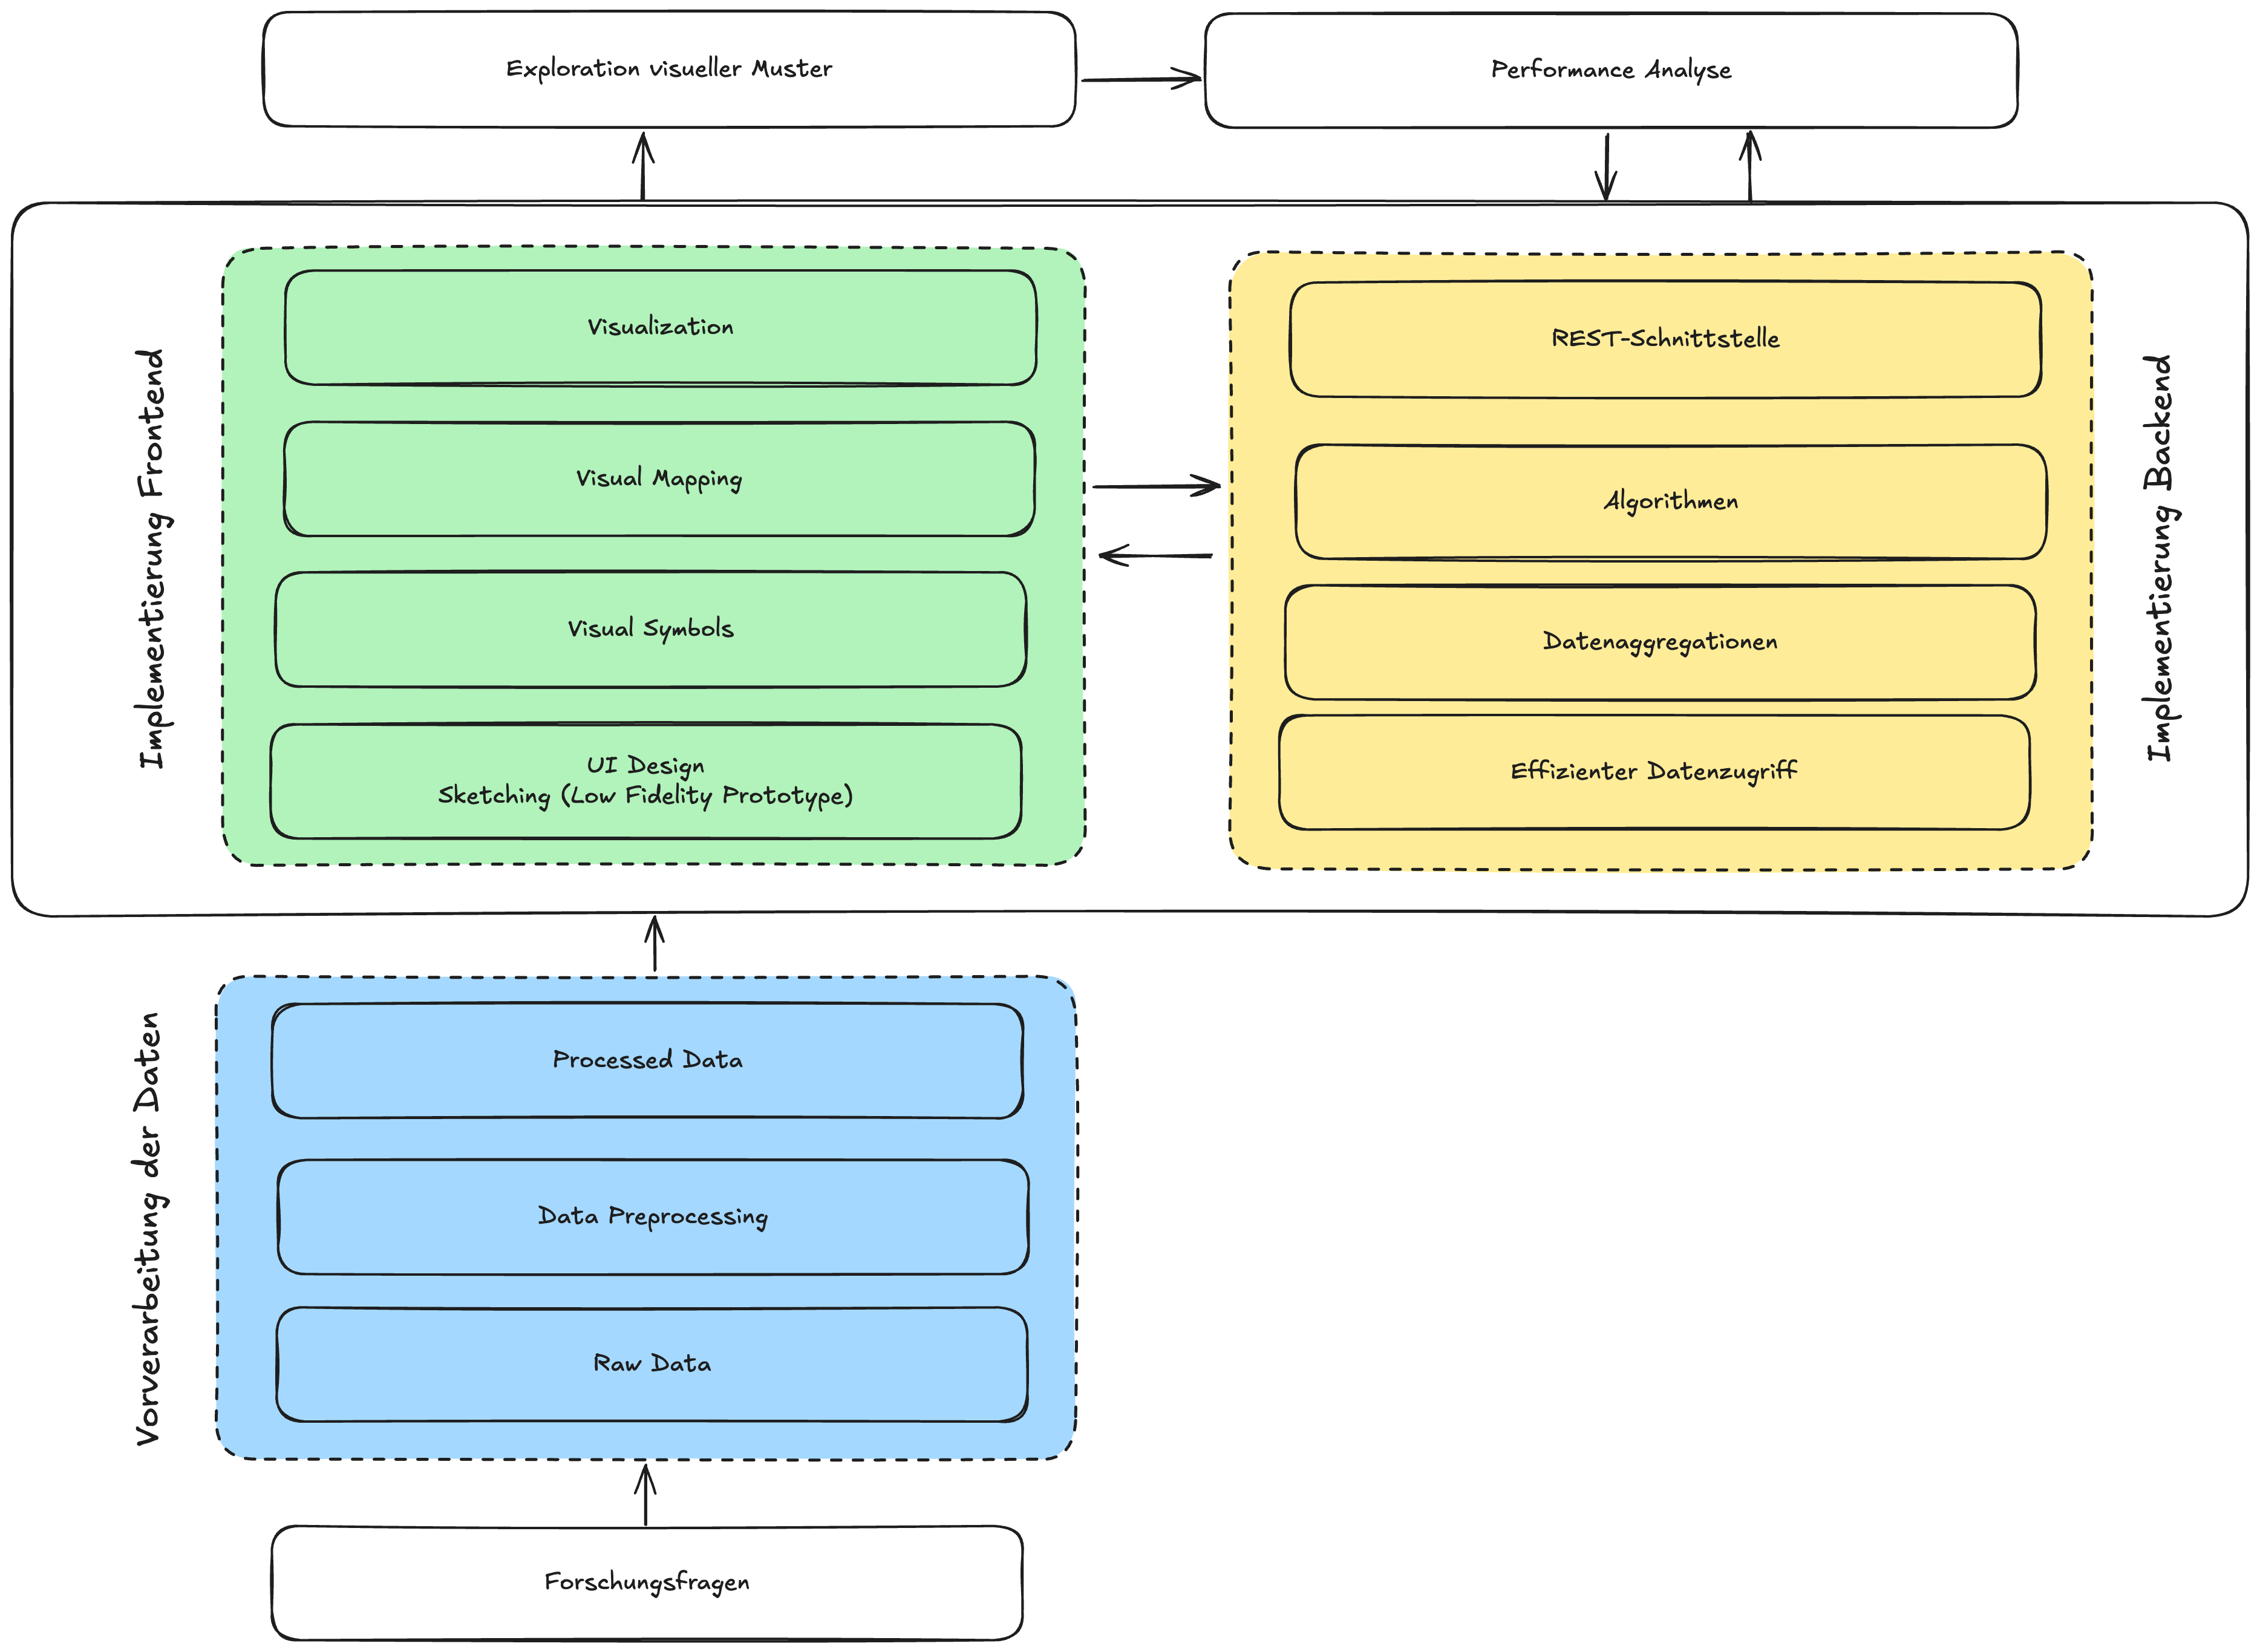
\includegraphics[width=.8\linewidth]{content/00_assets/vorgehen.png}
    \label{fig_vorgehen}
\end{figure}


Das VA-Tool selbst wird aus drei Hauptbestandteilen aufgebaut, einem \textit{Frontend}, einem \textit{Backend}, sowie einer \textit{\acrfull{rest} API}. Das \textbf{Frontend} ist hierbei für die Visualisierung der Daten sowie die Handhabung der Nutzerinteraktionen zuständig. Das \textbf{Backend} ist für die notwendigen Algorithmen und die Datenabfragen verantwortlich. Das Frontend und Backend kommunizieren miteinander über eine  \acrshort{rest} Schnittstelle (siehe Abbildung \ref{fig_va_tool_design}). Diese Trennung hat den Vorteil, dass die Visualisierungslogik von der Anwenderlogik getrennt ist und somit die Visualisierungslogik unabhängig von der Anwendungslogik ausgetauscht werden kann.

\begin{figure}[H]
    \caption{Technischer Aufbau des VA-Tools (eigene Darstellung)}
    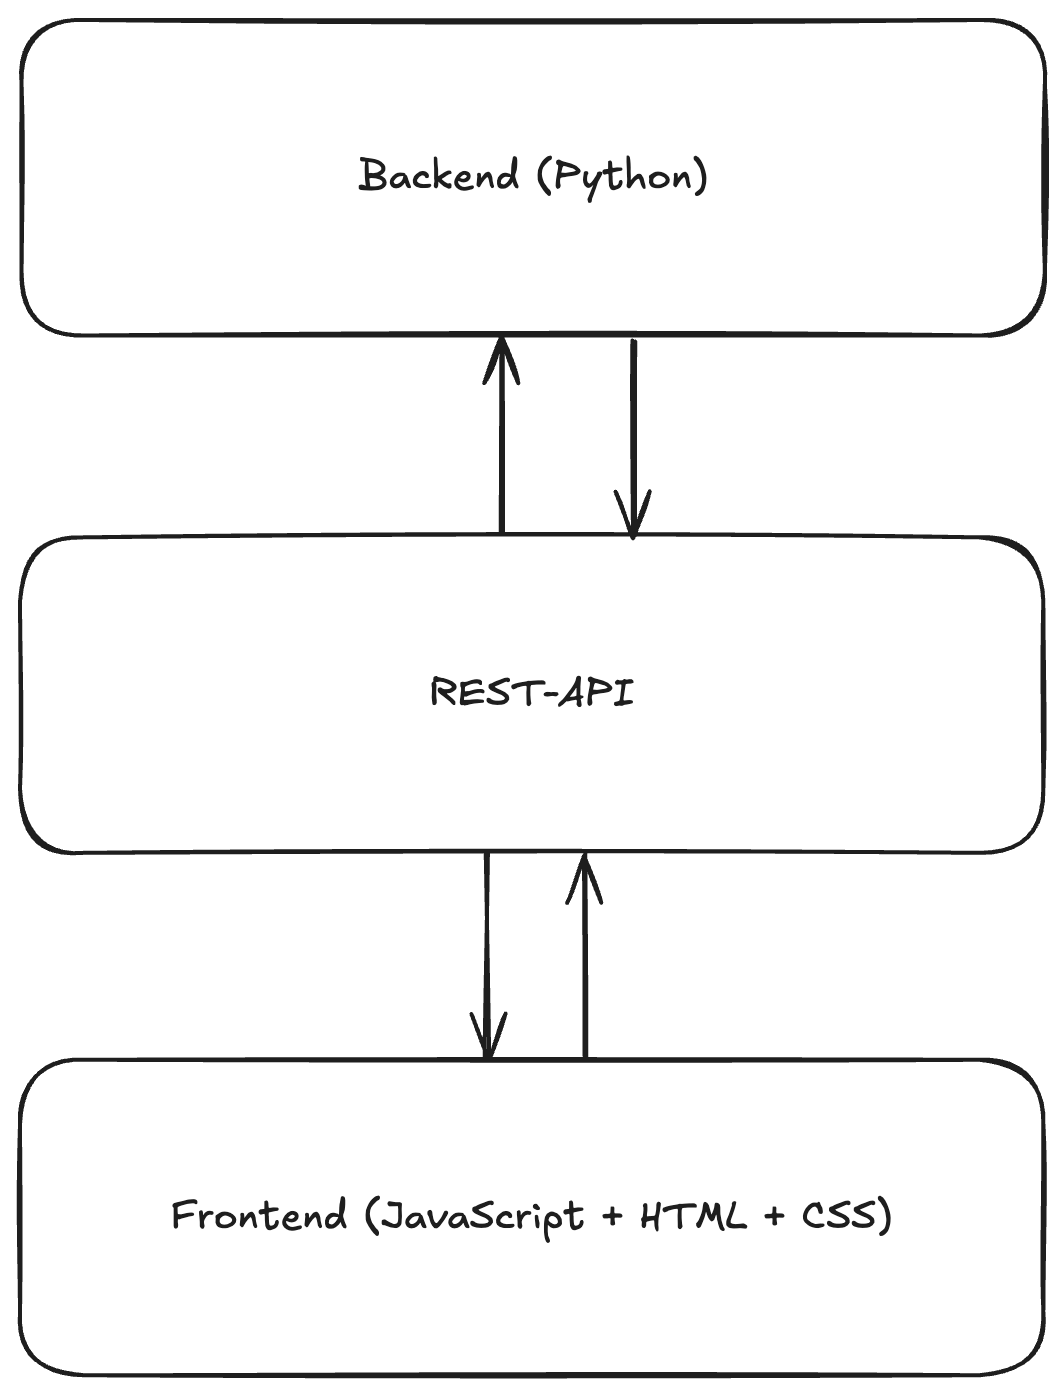
\includegraphics[width=.3\linewidth]{content/00_assets/aufbau_va_tool.png}
    \label{fig_va_tool_design}
\end{figure}

Nachfolgend wird auf die wichtigsten Elemente gemäss Abbildung \ref{fig_vorgehen} eingegangen.

\section{Vorverarbeitung der Daten}
Ausgehend von den Forschungsfragen werden die Datenquellen evaluiert und entsprechend aufbereitet.

\subsection{Raw Data}
Als Datengrundlage dienen die öffentlich zugänglichen Daten der SBB auf Open Data\footnote{\url{https://data.sbb.ch/pages/home/}}. Als Hauptdatenquelle wird die Gegenüberstellung von Zielankunftszeit zu den effektiven Ankunftszeiten verwendet\footnote{\url{https://data.sbb.ch/explore/dataset/actual-data-sbb-previous-day/information/}}. Hieraus lassen sich die Verspätungen pro Station und Zuglinie ermitteln. Als weitere Datenquellen wird das Betriebspunktenetz\footnote{\url{https://data.sbb.ch/explore/dataset/linie-mit-betriebspunkten/information/}} verwendet. Weitere Datenquellen werden im Verlaufe der Arbeit, soweit sinnvoll, hinzugenommen.

\subsection{Data Preprocessing}
Innerhalb des Data Preprocessing werden die Daten optimal zur Beantwortung der Forschungsfragen aufbereitet. Hierunter fallen insbesondere das Data Cleaning sowie evtl. notwendige Daten-Aggregationen. Um sicherzustellen, dass einfach neue Datensätze eingebunden werden können, wird ein entsprechendes Python-Script geschrieben, welches das Data Preprocessing automatisiert.

\subsection{Processed Data}
Die vorverarbeiteten Daten werden optimal für einen schnellen Zugriff gespeichert. Falls notwendig, werden  Datenbanksysteme speziell für analytische Datenauswertungen wie DuckDB verwendet.

\section{Implementierung Frontend und Backend}
Sowohl Frontend und Backend werden parallel entwickelt. Dies ist notwendig um die Daten, welche das Backend liefert, dem Nutzer zu visualisieren, als auch um auf bestimmte Nutzerinteraktionen (Filterung, Anpassung der Parameter) zu reagieren und gegebenenfalls die Algorithmen anzupassen.

\subsection{Frontend}
Ausgehend von den Forschungsfragen sowie den vorverarbeiteten Daten wird ein Low Fidelity Prototyp des VA-Tools in Form einer Skizze erstellt. Aufgrund der Skizze werden anschliessend die Visual Symbols (Liniendiagramme etc.) umgesetzt. Um möglichst viele Endnutzer zu erreichen, wird das Frontend als Web-Applikation mittels JavaScript, HTML und CSS entwickelt.

\subsection{Backend}
Das Backend beinhaltet die komplette Algorithmik und ist für einen effizienten Datenzugriff und entsprechende Datenaggregation notwendig. Bei den Algorithmen werden verschiedene Cluster-Algorithmen evaluiert (bspw. K-Means für räumliches Clustering). Teil des Backends ist auch die Implementierung einer \acrshort{rest} Schnittstelle.

\section{Exploration visueller Muster und Performance Analyse}
Nachdem das Frontend sowie Backend erstellt wurden, können die visuellen Muster mithilfe des VA-Tools exploriert werden. Um eine effiziente Exploration zu ermöglichen, wird auch eine Performance-Analyse durchgeführt, was wiederum Anpassungen am Front- sowie Backend mit sich führen kann.
